\section{Introduction}
\label{sec:intro}

Pairwise TTC surrogates characterize instantaneous criticality between two actors, while recorded driving scenes contain additional nearby actors and contextual conditions~\cite{hayward1972near,minderhoud2001extended,ettinger2021large,westhofen2023criticality}. Such a reduction is interpretable, but it may omit measurable information carried by other nearby actors, traffic composition, and roadway context~\cite{koopman2017challenges,iso34503,saej3016}. We therefore ask a narrower evaluation question: after controlling for a clean nearest-clearance SDC--actor representation, do dataset-observable current-frame ODD-context proxies improve identification of ego-centric minimum swept OBB-TTC events, and are the resulting proxy associations coherent with temporal target profiles?

\begin{figure*}[t]
\centering
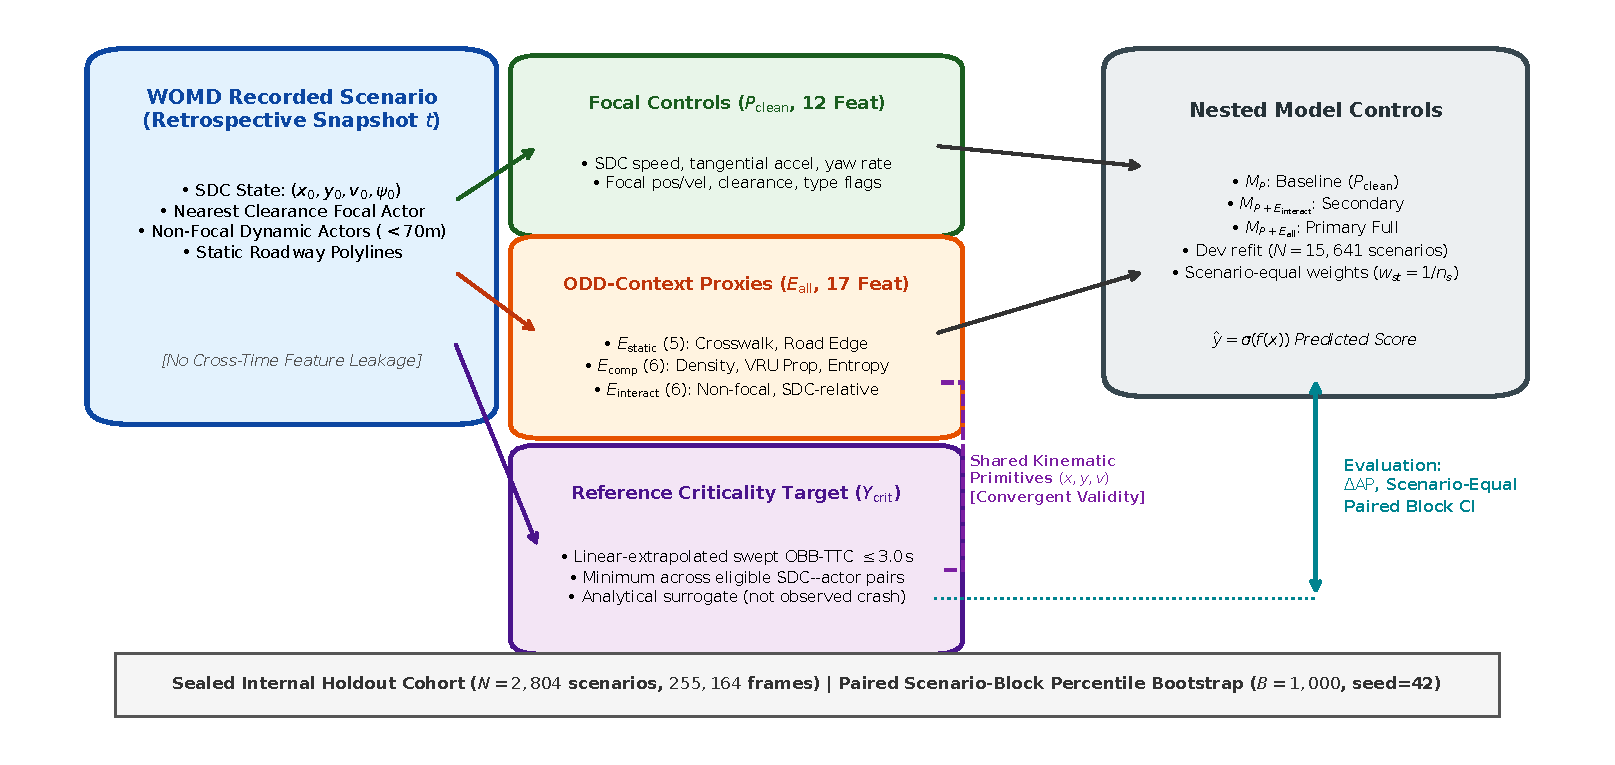
\includegraphics[width=0.98\textwidth]{figures/fig1_measurement_architecture.pdf}
\caption{\textbf{Evaluation Architecture and Construct Boundaries.} Overview of the construct-controlled, scenario-disjoint audit protocol. Retrospective snapshot frames extract clean focal physical kinematics ($P_{\text{clean}}$, 12 features) and observable operational-context proxies ($E_{\text{all}}$, 17 features). Nested gradient-boosted models are evaluated against an ego-centric minimum swept SAT OBB-TTC reference target across eligible dynamic actors within 70 m on a sealed one-shot holdout cohort ($N=255,164$ frames).}
\label{fig:measurement_arch}
\end{figure*}

Our contributions are threefold:
\begin{enumerate}
    \item \textbf{Construct-Controlled Audit Formulation}: We define a construct-controlled current-frame audit that compares a nearest-clearance focal baseline with nested ODD-context proxy families for an ego-centric all-nearby-actor TTC target; the target, proxy, and shared-state boundaries are explicit.
    \item \textbf{Sealed Holdout Incremental Finding}: We apply a scenario-disjoint one-shot holdout protocol with scenario-equal metrics and paired scenario-block bootstrap inference, finding a supported but modest full-context increment ($\Delta\text{AP} = +0.0147$, $95\%$ CI $[+0.0005, +0.0285]$). The protocol limits post-hoc tuning, preserves scenario disjointness, and makes the single holdout access auditable.
    \item \textbf{Feature-Family and Temporal Completeness Evidence}: Family-restricted comparisons and development-to-holdout feature confirmation provide secondary localization evidence, while residualized scenario-profile analyses test temporal completeness against target Peak, AUC, and TET3. Warp experiments remain excluded and within-dataset vehicle-response KPIs are reported only as supportive development evidence.
\end{enumerate}
